\documentclass[journal,12pt,twocolumn]{IEEEtran}
%
\usepackage{setspace}
\usepackage{gensymb}
%\doublespacing
\singlespacing

%\usepackage{graphicx}
%\usepackage{amssymb}
%\usepackage{relsize}
\usepackage[cmex10]{amsmath}
\usepackage{siunitx}
%\usepackage{amsthm}
%\interdisplaylinepenalty=2500
%\savesymbol{iint}
%\usepackage{txfonts}
%\restoresymbol{TXF}{iint}
%\usepackage{wasysym}
\usepackage{amsthm}
\usepackage{iithtlc}
\usepackage{mathrsfs}
\usepackage{txfonts}
\usepackage{stfloats}
\usepackage{steinmetz}
\usepackage{supertabular}
%\usepackage{bm}
\usepackage{cite}
\usepackage{cases}
\usepackage{subfig}
%\usepackage{xtab}
\usepackage{longtable}
\usepackage{multirow}
%\usepackage{algorithm}
%\usepackage{algpseudocode}
\usepackage{enumitem}
\usepackage{mathtools}
\usepackage{tikz}
\usepackage{circuitikz}
\usepackage{verbatim}
\usepackage{tfrupee}
\usepackage[breaklinks=true]{hyperref}
%\usepackage{stmaryrd}
\usepackage{tkz-euclide} % loads  TikZ and tkz-base
%\usetkzobj{all}
\usetikzlibrary{calc,math}
\usetikzlibrary{fadings}
\usepackage{listings}
    \usepackage{color}                                            %%
    \usepackage{array}                                            %%
    \usepackage{longtable}                                        %%
    \usepackage{calc}                                             %%
    \usepackage{multirow}                                         %%
    \usepackage{hhline}                                           %%
    \usepackage{ifthen}                                           %%
  %optionally (for landscape tables embedded in another document): %%
    \usepackage{lscape}     
\usepackage{multicol}
\usepackage{chngcntr}
\usepackage{blkarray}
\usepackage{karnaugh-map}
\usepackage{fontspec}
\usepackage[intoc]{nomencl}
\makenomenclature

%\usetikzlibrary{arrows, shapes.gates.logic.US, calc}
\usetikzlibrary{arrows,shapes.gates.logic.US,shapes.gates.logic.IEC,calc}
\setmainfont[ Path = fonts/]{Sanskrit_2003.ttf}
%\setmainfont{Sanskrit_2003.ttf}
%\setmainfont{Nakula.ttf}
%\setmainfont{Lohit-Devanagari.ttf}


%\usepackage{enumerate}

%\usepackage{wasysym}
%\newcounter{MYtempeqncnt}
\DeclareMathOperator*{\Res}{Res}
%\renewcommand{\baselinestretch}{2}
\renewcommand\thesection{\arabic{section}}
\renewcommand\thesubsection{\thesection.\arabic{subsection}}
\renewcommand\thesubsubsection{\thesubsection.\arabic{subsubsection}}

\renewcommand\thesectiondis{\arabic{section}}
\renewcommand\thesubsectiondis{\thesectiondis.\arabic{subsection}}
\renewcommand\thesubsubsectiondis{\thesubsectiondis.\arabic{subsubsection}}

% correct bad hyphenation here
\hyphenation{op-tical net-works semi-conduc-tor}
\def\inputGnumericTable{}                                 %%


\lstset{
%language=shell,
%language = Prolog,
frame=single, 
breaklines=true,
%showstringspaces=false,
columns=fullflexible
literate = {-}{-}1
}
%\lstset{
%language=tex,
%frame=single, 
%breaklines=true
%}

\begin{document}
%


\newtheorem{theorem}{Theorem}[section]
\newtheorem{problem}{Problem}
\newtheorem{proposition}{Proposition}[section]
\newtheorem{lemma}{Lemma}[section]
\newtheorem{corollary}[theorem]{Corollary}
\newtheorem{example}{Example}[section]
\newtheorem{definition}[problem]{Definition}
%\newtheorem{thm}{Theorem}[section] 
%\newtheorem{defn}[thm]{Definition}
%\newtheorem{algorithm}{Algorithm}[section]
%\newtheorem{cor}{Corollary}
\newcommand{\BEQA}{\begin{eqnarray}}
\newcommand{\EEQA}{\end{eqnarray}}
\newcommand{\define}{\stackrel{\triangle}{=}}

\bibliographystyle{IEEEtran}
%\bibliographystyle{ieeetr}


\providecommand{\mbf}{\mathbf}
\providecommand{\pr}[1]{\ensuremath{\Pr\left(#1\right)}}
\providecommand{\qfunc}[1]{\ensuremath{Q\left(#1\right)}}
\providecommand{\sbrak}[1]{\ensuremath{{}\left[#1\right]}}
\providecommand{\lsbrak}[1]{\ensuremath{{}\left[#1\right.}}
\providecommand{\rsbrak}[1]{\ensuremath{{}\left.#1\right]}}
\providecommand{\brak}[1]{\ensuremath{\left(#1\right)}}
\providecommand{\lbrak}[1]{\ensuremath{\left(#1\right.}}
\providecommand{\rbrak}[1]{\ensuremath{\left.#1\right)}}
\providecommand{\cbrak}[1]{\ensuremath{\left\{#1\right\}}}
\providecommand{\lcbrak}[1]{\ensuremath{\left\{#1\right.}}
\providecommand{\rcbrak}[1]{\ensuremath{\left.#1\right\}}}
\providecommand{\ceil}[1]{\left \lceil #1 \right \rceil }
\theoremstyle{remark}
\newtheorem{rem}{Remark}
\newcommand{\sgn}{\mathop{\mathrm{sgn}}}
\providecommand{\abs}[1]{\left\vert#1\right\vert}
\providecommand{\res}[1]{\Res\displaylimits_{#1}} 
\providecommand{\norm}[1]{\left\lVert#1\right\rVert}
%\providecommand{\norm}[1]{\lVert#1\rVert}
\providecommand{\mtx}[1]{\mathbf{#1}}
\providecommand{\mean}[1]{E\left[ #1 \right]}
\providecommand{\fourier}{\overset{\mathcal{F}}{ \rightleftharpoons}}
%\providecommand{\hilbert}{\overset{\mathcal{H}}{ \rightleftharpoons}}
\providecommand{\system}{\overset{\mathcal{H}}{ \longleftrightarrow}}
	%\newcommand{\solution}[2]{\textbf{Solution:}{#1}}
\newcommand{\solution}{\noindent \textbf{Solution: }}
\newcommand{\cosec}{\,\text{cosec}\,}
\providecommand{\dec}[2]{\ensuremath{\overset{#1}{\underset{#2}{\gtrless}}}}
\newcommand{\myvec}[1]{\ensuremath{\begin{pmatrix}#1\end{pmatrix}}}
\newcommand{\mydet}[1]{\ensuremath{\begin{vmatrix}#1\end{vmatrix}}}
%\numberwithin{equation}{section}
\numberwithin{equation}{subsection}
%\numberwithin{problem}{section}
%\numberwithin{definition}{section}
\makeatletter
\@addtoreset{figure}{problem}
\makeatother

\let\StandardTheFigure\thefigure
\let\vec\mathbf
%\renewcommand{\thefigure}{\theproblem.\arabic{figure}}
%\renewcommand{\thefigure}{\theproblem}
\renewcommand{\thefigure}{\thesection}
%\setlist[enumerate,1]{before=\renewcommand\theequation{\theenumi.\arabic{equation}}
%\counterwithin{equation}{enumi}


%\renewcommand{\theequation}{\arabic{subsection}.\arabic{equation}}

\def\putbox#1#2#3{\makebox[0in][l]{\makebox[#1][l]{}\raisebox{\baselineskip}[0in][0in]{\raisebox{#2}[0in][0in]{#3}}}}
     \def\rightbox#1{\makebox[0in][r]{#1}}
     \def\centbox#1{\makebox[0in]{#1}}
     \def\topbox#1{\raisebox{-\baselineskip}[0in][0in]{#1}}
     \def\midbox#1{\raisebox{-0.5\baselineskip}[0in][0in]{#1}}

\vspace{3cm}

\title{
%	\logo{
Introduction to ARM-GCC using Pygmy
%	}
}
\author{ 
%गाड़ेपल्लि वेंकट विश्वनाथ शर्मा $^{*}$% <-this % stops a space
%	\thanks{*रचयिता भारतीय प्रौद्योगिकी संस्थान, हैदराबाद,५०२२८५ के विद्युत अभियान्त्रिकी विभाग में कार्यरत हैं, ईमेल:gadepall@ee.iith.ac.in। यह लेख मुक्त स्रोत विचारधारा के अनुरूप  है।}
G V V Sharma$^{*}$% <-this % stops a space
	\thanks{*The author is with the Department of Electrical Engineering, IIT Hyderabad, 502285. email:gadepall@ee.iith.ac.in। All content in this manual is released under GNU/GPL.}
	
}	
%\title{
%	\logo{Matrix Analysis through Octave}{\begin{center}\includegraphics[scale=.24]{tlc}\end{center}}{}{HAMDSP}
%}


% paper title
% can use linebreaks \\ within to get better formatting as desired
%\title{Matrix Analysis through Octave}
%
%
% author names and IEEE memberships
% note positions of commas and nonbreaking spaces ( ~ ) LaTeX will not break
% a structure at a ~ so this keeps an author's name from being broken across
% two lines.
% use \thanks{} to gain access to the first footnote area
% a separate \thanks must be used for each paragraph as LaTeX2e's \thanks
% was not built to handle multiple paragraphs
%

%\author{<-this % stops a space
%\thanks{}}
%}
% note the % following the last \IEEEmembership and also \thanks - 
% these prevent an unwanted space from occurring between the last author name
% and the end of the author line. i.e., if you had this:
% 
% \author{....lastname \thanks{...} \thanks{...} }
%                     ^------------^------------^----Do not want these spaces!
%
% a space would be appended to the last name and could cause every name on that
% line to be shifted left slightly. This is one of those "LaTeX things". For
% instance, "\textbf{A} \textbf{B}" will typeset as "A B" not "AB". To get
% "AB" then you have to do: "\textbf{A}\textbf{B}"
% \thanks is no different in this regard, so shield the last } of each \thanks
% that ends a line with a % and do not let a space in before the next \thanks.
% Spaces after \IEEEmembership other than the last one are OK (and needed) as
% you are supposed to have spaces between the names. For what it is worth,
% this is a minor point as most people would not even notice if the said evil
% space somehow managed to creep in.



% The paper headers
%\markboth{Journal of \LaTeX\ Class Files,~Vol.~6, No.~1, January~2007}%
%{Shell \MakeLowercase{\textit{et al.}}: Bare Demo of IEEEtran.cls for Journals}
% The only time the second header will appear is for the odd numbered pages
% after the title page when using the twoside option.
% 
% *** Note that you probably will NOT want to include the author's ***
% *** name in the headers of peer review papers.                   ***
% You can use \ifCLASSOPTIONpeerreview for conditional compilation here if
% you desire.




% If you want to put a publisher's ID mark on the page you can do it like
% this:
%\IEEEpubid{0000--0000/00\$00.00~\copyright~2007 IEEE}
% Remember, if you use this you must call \IEEEpubidadjcol in the second
% column for its text to clear the IEEEpubid mark.



% make the title area
\maketitle

\newpage

\tableofcontents


\bigskip

%\renewcommand{\thefigure}{\theenumi}
%\renewcommand{\thetable}{\theenumi}
%\renewcommand{\abstractname}{सार}
%\renewcommand{\nomname}{नामकरण}
%\renewcommand{\solution}{हल: }
%\renewcommand{\figurename}{आकृति.}
%\renewcommand{\tablename}{सारणी.}
%\renewcommand{\theequation}{\theenumi}

%\begin{abstract}
%%\boldmath
%In this letter, an algorithm for evaluating the exact analytical bit error rate  (BER)  for the piecewise linear (PL) combiner for  multiple relays is presented. Previous results were available only for upto three relays. The algorithm is unique in the sense that  the actual mathematical expressions, that are prohibitively large, need not be explicitly obtained. The diversity gain due to multiple relays is shown through plots of the analytical BER, well supported by simulations. 
%
%\end{abstract}
% IEEEtran.cls defaults to using nonbold math in the Abstract.
% This preserves the distinction between vectors and scalars. However,
% if the journal you are submitting to favors bold math in the abstract,
% then you can use LaTeX's standard command \boldmath at the very start
% of the abstract to achieve this. Many IEEE journals frown on math
% in the abstract anyway.

% Note that keywords are not normally used for peerreview papers.
%\begin{IEEEkeywords}
%Cooperative diversity, decode and forward, piecewise linear
%\end{IEEEkeywords}



% For peer review papers, you can put extra information on the cover
% page as needed:
% \ifCLASSOPTIONpeerreview
% \begin{center} \bfseries EDICS Category: 3-BBND \end{center}
% \fi
%
% For peerreview papers, this IEEEtran command inserts a page break and
% creates the second title. It will be ignored for other modes.
%\IEEEpeerreviewmaketitle

\begin{abstract}
This document provides a simple introduction to ARM programming using Pygmy.
%इस लेख में  वामन  के द्वारा आर्म-क्रमादेशन  से छात्रों का परिचय कराया जाएगा।


%ॐ श्री गणेशाय नमः॥
%\\
%\indent जय श्री राम।
%This manual provides a simple introduction to Digital Design.
\end{abstract}

%\section{Nomenclature}
%\printnomenclature[1.7in]
%%\addcontentsline{toc}{chapter}{Nomenclature}

%\nomenclature{Seven Segment Display}{ सप्तांश प्रदर्शी} 
%\nomenclature{Code}{ गूढ़} 
%\nomenclature{Decoder}{ गूढ़वाचक}
%\nomenclature{Incrementing}{ परवर्ती}
%\nomenclature{Decrementing}{ पूर्ववर्ती}
%\nomenclature{Karnaugh Map}{ कार्नो मानचित्र}
%\nomenclature{Implicant}{ विवक्षक}
%\nomenclature{LED}{ प्रकाश उत्सर्जक यंत्र}
%\nomenclature{Table}{ सारणी}
%\nomenclature{Figure}{ आकृति}
%\nomenclature{Variable}{ चर}
%\nomenclature{Input}{ आगत}
%\nomenclature{Output}{ निर्गत}
%\nomenclature{Boolean Algebra}{ बूलीय बीजगणित}
%\nomenclature{Verify}{ सत्यापित}
%\nomenclature{Combinational Logic}{ संयोजक तर्क}
%\nomenclature{Minimize}{ कनिष्ठीकरण}
\nomenclature{Execute}{ निष्पादित, चालयन}
%\nomenclature{Expression}{ व्यंजक}
%\nomenclature{Equation}{ समीकरण}
%\nomenclature{Axiom}{ अभिगृह}
%\nomenclature{Reduced}{ समानयनिक}
%\nomenclature{C Program}{ C क्रमादेश}
\nomenclature{Programming}{  क्रमादेशन}
\nomenclature{Frequency}{ आवृत्ति}
\nomenclature{Bit length}{ मात्राभार}
\nomenclature{Cable}{ रज्जु}
\nomenclature{Button}{ गण्ड}
\nomenclature{Left}{ वाम}
\nomenclature{Right}{दक्षिण}
\nomenclature{Blink}{श्मील}
\nomenclature{IP Address}{अनिकेत}
\nomenclature{Send}{प्रेषण}
\nomenclature{File}{सञ्चिका}
\nomenclature{Setup}{सप्रतिष्ठान}
%\nomenclature{Execute}{चालयन}
\nomenclature{Interval}{अंतराल}

%\nomenclature{Binary}{ द्विआधारी}
%\nomenclature{Truth Table}{सत्य सारणी}
%\nomenclature{Derive}{व्युत्पन्न }
%\nomenclature{XOR}{अर्ध योग}
%\nomenclature{Complement}{पूरक}
%\nomenclature{Decade Counter}{दशक गणित्र}
%\nomenclature{Digital Logic}{अंकीय तर्क}
%\nomenclature{Function}{फलन}
%\nomenclature{Block Diagram}{खण्डारेख}
%\nomenclature{Circuit}{परिपथ}
%\nomenclature{Simplified Expression}{सरलीकृत व्यंजक}
\nomenclature{Delay}{अतिकाल}
\nomenclature{Minute}{निमिश}
%\nomenclature{Synchronous}{तुल्यकालिक}
%\nomenclature{Finite State Machine}{परिमित अवस्था यंत्र}
%\nomenclature{State Transition Table}{अवस्थान्तरण सारणी}
%\nomenclature{Flip flop}{द्विविध}
%\nomenclature{Design}{अभिकल्प}
%\nomenclature{Implementation}{कार्यान्वयन}
%\nomenclature{Period}{आवर्त}
\nomenclature{Hardware}{यंत्रान्श}
\nomenclature{Software}{तंंत्रान्श}
\nomenclature{Computer}{संगणक}
\nomenclature{Board}{परिपथफलक}
\nomenclature{Port}{पत्तन}
\nomenclature{Now}{इदान}
\nomenclature{Weblink}{जालबन्धन}
\nomenclature{Download}{अवाहरत}
\nomenclature{Resistance}{प्रतिरोध}
\nomenclature{Flash}{प्रस्फुरण}
\nomenclature{Wire}{तन्तु}







 


\section{Software}
%
All codes used in this document are available at the following link
%निम्न जालबन्धन से इस लिख में उपयोग किए गए समस्त क्रमादेश अवाहरत करें।
\begin{lstlisting}
https://github.com/gadepall/vaman/tree/master/arm/codes/setup
\end{lstlisting}


\section{Setup}
\renewcommand{\theequation}{\theenumi}
\renewcommand{\thefigure}{\theenumi}
\begin{enumerate}[label=\thesection.\arabic*.,ref=\thesection.\theenumi]
\numberwithin{equation}{enumi}
\numberwithin{figure}{enumi}
\numberwithin{table}{enumi}

\item Connect the raspberry pi to pygmy through USB.
\item On the left of the USB port, an LED and a button can be seen.  Another button is visible on
the right of the USB port.
\item Press the right button and immediately press the left button.  The green LED starts blinking.  The pygmy is now in download mode.
mode.
%दक्षिण गण्ड को दबाकर शीघ्र वाम गण्ड को दबायें।  हरित दीप श्मीलित होते हुए दिखेगा।  यह संकेत हैं कि वामन
%क्रमादेश के लिए सिद्ध है।

\item Open termux on android and execute the following codes
\begin{lstlisting}
cd ~
svn co https://github.com/gadepall/vaman/trunk/arm/codes/setup/blink
cd GCC_Project
make
scp  output/bin/blink.bin pi@192.168.0.114:
\end{lstlisting}
Appropriately modify the above ip address before sending blink.bin to the pi.
% सञ्चिका प्रेषण पूर्व रास्पबेरी पै का उचित अनिकेत दें। 
\item Now log on to the RPi and execute teh following
%अब रास्पबेरी पै  में प्रवेश कर निम्न  आदेश का चालयन करें
\begin{lstlisting}
sudo python3 /home/pi/pygmy-dev/pygmy-sdk/TinyFPGA-Programmer-Application/tinyfpga-programmer-gui.py --port /dev/ttyACM0  --m4app  blink.bin --mode m4-fpga
\end{lstlisting}
\item Enter the appropriate USB device port above while executing.  Press the button to the right
after the above command is successfully executed.  The LED will start blinking. 
%उपरोक्त आदेश में उचित पत्तन दें। तत्पश्चात यूएसबी पत्तन के दक्षिण दिशा में गण्ड को दबायें। कुछ समय पश्चचात प्रकाश उत्सर्जक श्वेत रंग  में श्मीलित होगा। 
\end{enumerate}
%
\section{Delay}

\renewcommand{\theequation}{\theenumi}
\renewcommand{\thefigure}{\theenumi}
\begin{enumerate}[label=\thesection.\arabic*.,ref=\thesection.\theenumi]
\numberwithin{equation}{enumi}
\numberwithin{figure}{enumi}
\numberwithin{table}{enumi}
\item See the following lines of the code below
\label{सम:क्रमादेश}
\begin{lstlisting}
codes/setup/blink/src/main.c
\end{lstlisting}
%की  इन पङ्क्तियों पर ध्यान दें । 
%
\begin{lstlisting}
    PyHal_Set_GPIO(18,1);//blue
    PyHal_Set_GPIO(21,1);//green
    PyHal_Set_GPIO(22,1);//red
        HAL_DelayUSec(2000000);
    PyHal_Set_GPIO(18,0);
    PyHal_Set_GPIO(21,0);
    PyHal_Set_GPIO(22,0);
\end{lstlisting}
%
We may conclude that the blink delay is 2000 000us = 2 s.
%इससे हम ज्ञात कर सकते हैं की वामन के दीप का शमीलनकाल 2000 000us = 2 s।  
\item Replace the following line in \ref{सम:क्रमादेश}  
\label{सम:द्विआधार}
\begin{lstlisting}
        HAL_DelayUSec(2000000);
\end{lstlisting}
%
with
\begin{lstlisting}
        HAL_DelayUSec(1000000);
\end{lstlisting}
and execute.  Can you see any difference in the blink period?
%से प्रतिस्थापित कर क्रमादेश का चालयन करें ।  क्या श्मीलनकाल में कोई परिवर्तन द्रश्य है?
\item To obtain red colour, execute the following code.
%रक्तिम रंगोत्पदन के लिए निम्न गूढ़ का चालयन करें।  
\begin{lstlisting}
codes/setup/red/src/main.c
\end{lstlisting}
Now obtain blue colour.
%इदान हरित एवं नील रंग में दीप को श्मीलित करें।

\item Now obtain green colour without blink.
%इदान  आर्म-जीसीसी  के द्वारा दीप में स्थायी रूप से  हरित वर्ण को उपलब्ध करें।
\\
\solution Execute the following code.
\begin{lstlisting}
codes/setup/onoff/src/main.c
\end{lstlisting}
%
\item  Using Table  \ref{table:input} and Fig.  \ref{fig:pin_sheet}, use an input pin to control the onboard LED.  
%एक अन्य कुश को निर्गत रूप देकर किसी बाह्य दीप को प्रकाशोर्जित करें.

\begin{table}[]
\centering
\begin{tabular}{|l|l|l|}
\hline
Type & Pin  &  Destination\\ \hline
Input &  IO\_5 &  GND\\ \hline
%आगत &  IO\_28 &  GND\\ \hline
%निर्गत  & IO\_11  &  LED\\ \hline
\end{tabular}
\caption{Pygmy control through external input.}
\label{table:input}
\end{table}

\begin{figure*}[!ht]
\centering
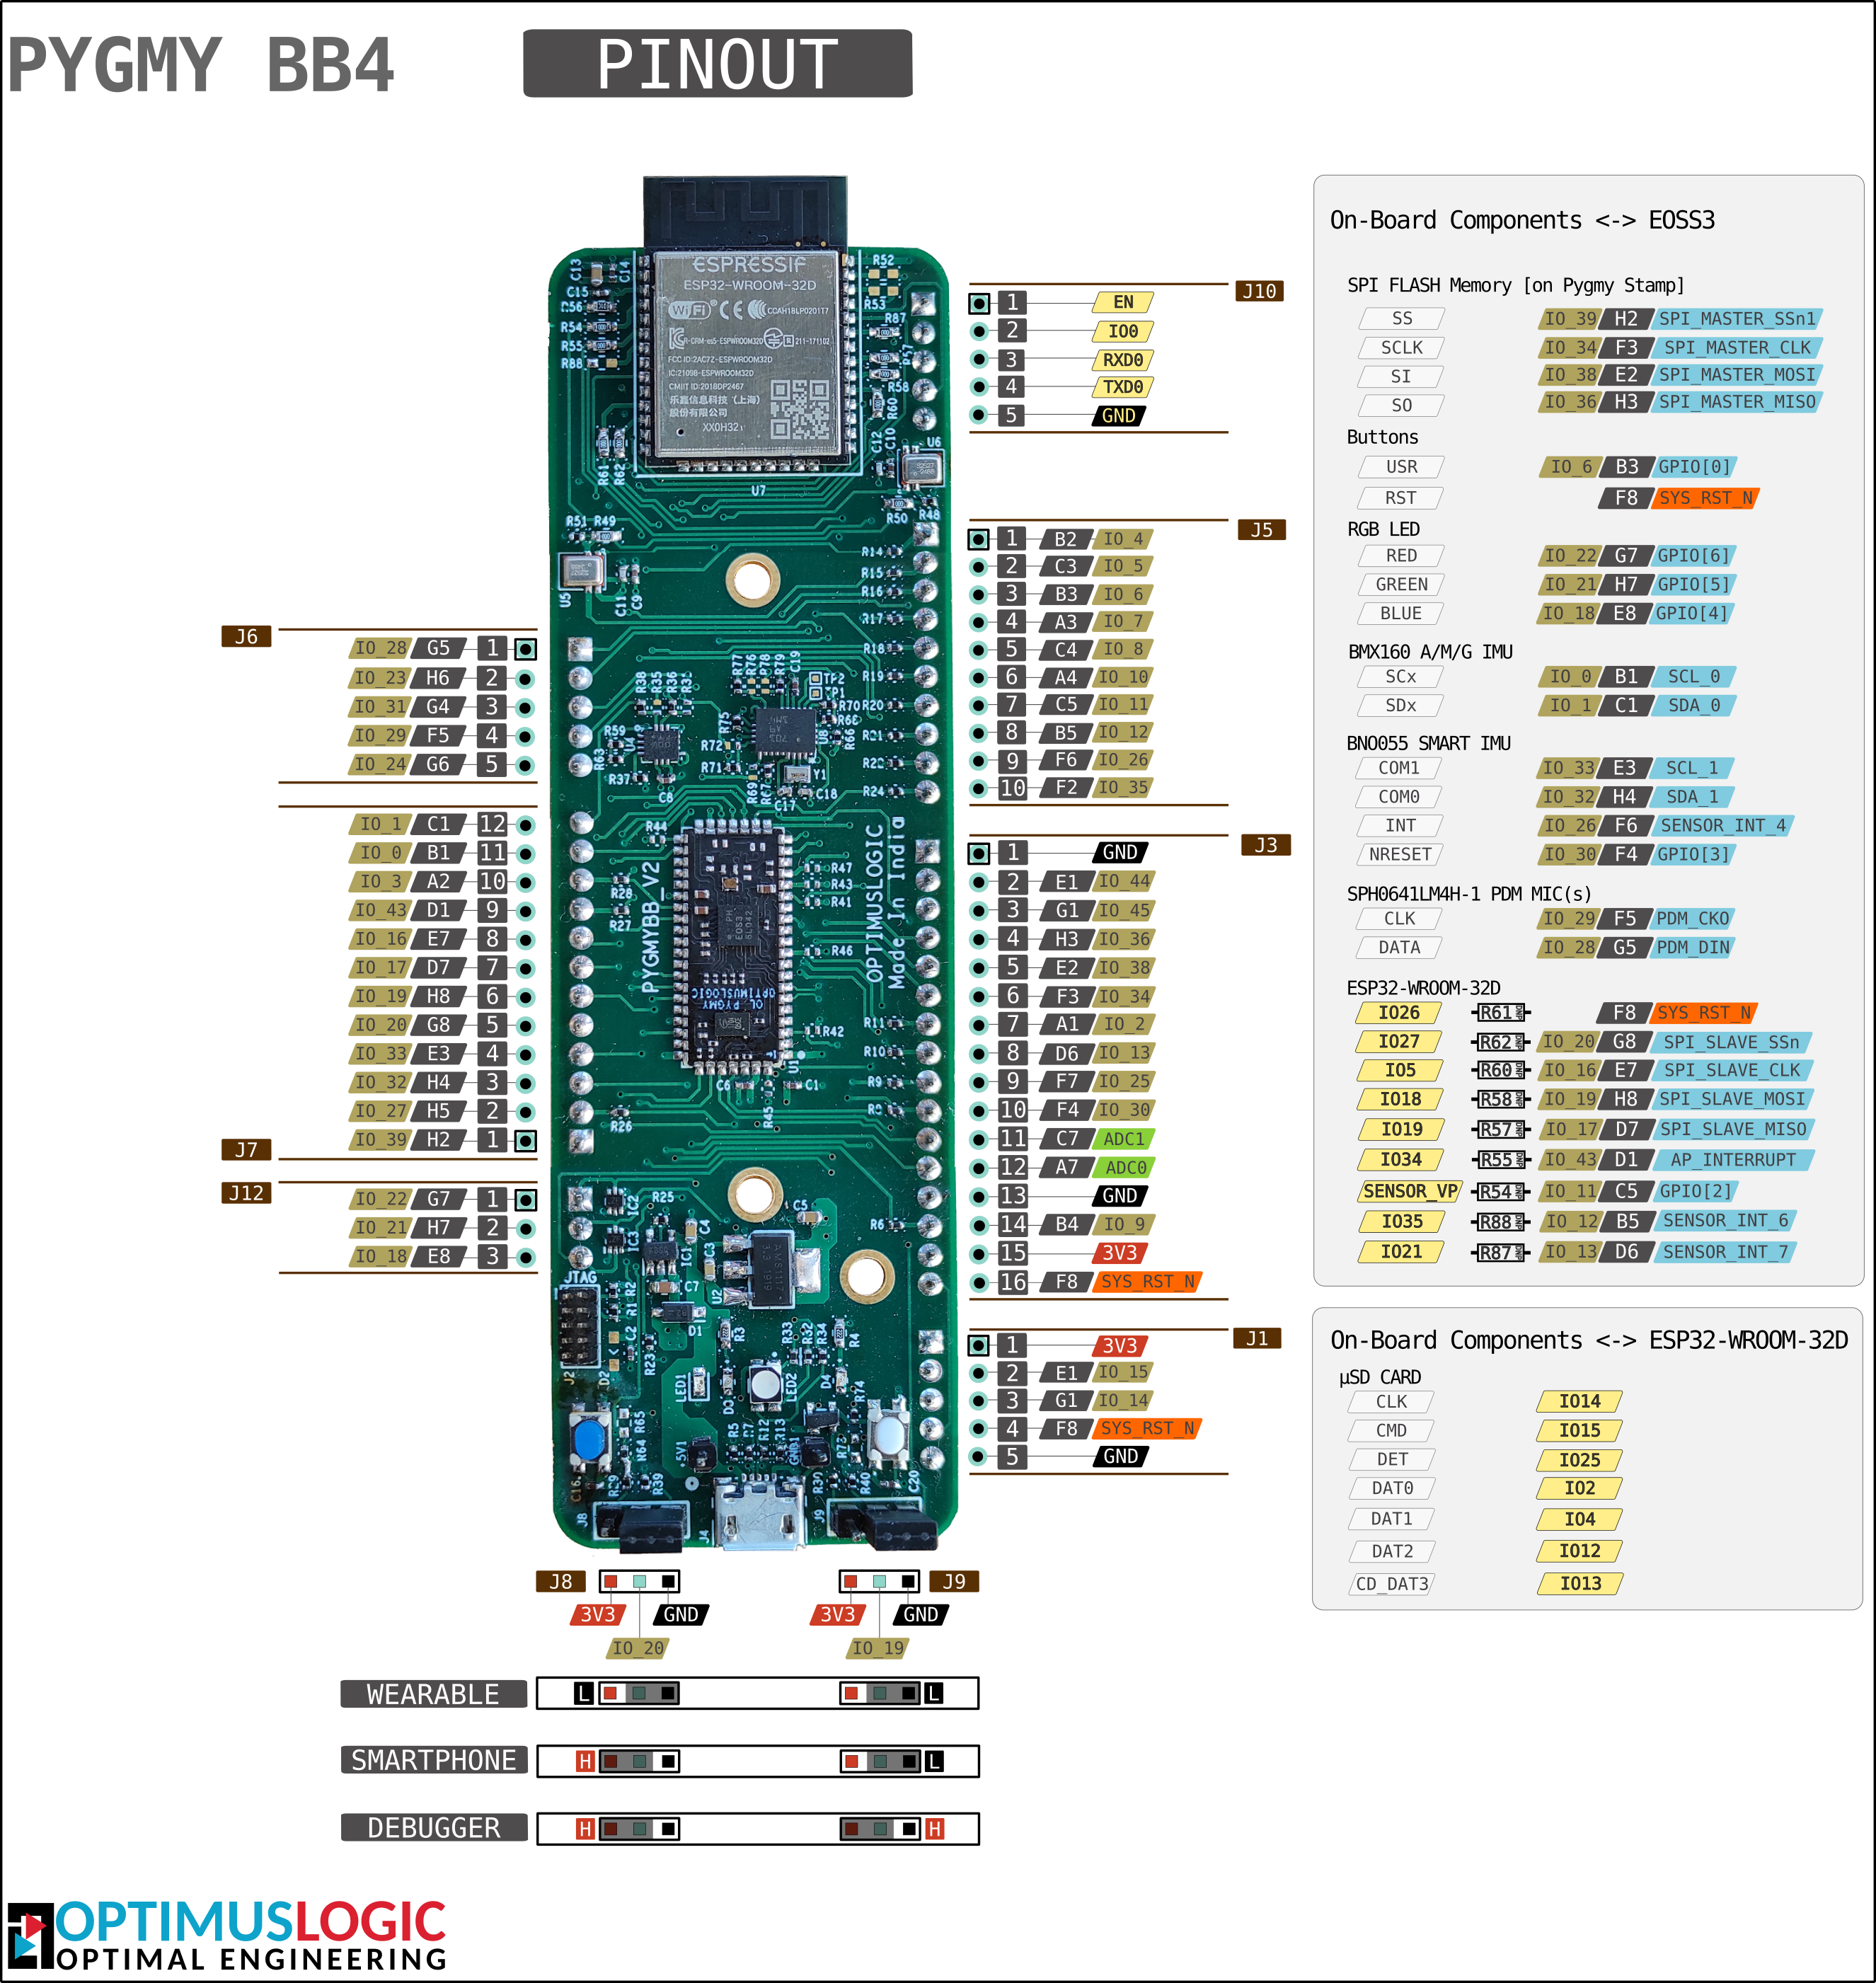
\includegraphics[width = \textwidth]{figs/pin_sheet.png}
\caption{Pin Diagram}
\label{fig:pin_sheet}
\end{figure*}
\solution Execute the following code.  You should see the LED blinking pink. Disconnecting the wire from GND will result in the LED blinking white 
and green alternately.
\begin{lstlisting}
codes/setup/gpio/src/main.c
\end{lstlisting}

\end{enumerate}
\end{document}



